\documentclass[conference,10pt,a4paper]{IEEEtran}
\usepackage[utf8]{inputenc}
\usepackage[T1]{fontenc}
\usepackage{amsmath,amssymb,amsfonts}
\usepackage{graphicx}
\usepackage{booktabs}
\usepackage{microtype}
\usepackage{hyperref}
\usepackage{tabularx}
\usepackage{cite}
\usepackage{balance}

\hypersetup{
    colorlinks=true,
    linkcolor=blue,
    citecolor=blue,
    urlcolor=blue
}

\title{Evaluating Lightweight Vision-Language and OCR Models on Occluded Document Images}

\author{\IEEEauthorblockN{Natural Language Processing Benchmark Study}
\IEEEauthorblockA{\textit{Department of Computer Science} \\
\textit{Faculty of Information Technology} \\
Course: CSC15006 --- Introduction to Natural Language Processing}
}

\begin{document}

\maketitle

\begin{abstract}
Optical Character Recognition (OCR) in real-world digitization workflows frequently suffers from physical and synthetic occlusions, including ink smudges, rubber stamps, correction fluid, and physical burning. While modern multimodal Vision-Language Models (VLMs) demonstrate remarkable document understanding capabilities, their autoregressive decoding cost poses severe computational bottlenecks. Conversely, specialized pipeline OCR models exhibit near-instantaneous throughput but lack generative contextual prior. This study conducts an extensive comparative evaluation of five lightweight models across 22,103 page evaluations on the held-out test split of the Occluded Pages Restoration Benchmark (OPRB). We analyze transcription fidelity (CER, WER, Bag-of-Words F1), degradation across text versus non-text occlusions, robustness over varying occlusion densities, qualitative failure modes, and the Pareto efficiency frontier. Our empirical findings demonstrate that lightweight pipeline OCR (PaddleOCR PP-OCRv4, 12M parameters) achieves the lowest Character Error Rate (0.3956) with a 90$\times$ latency advantage (1.14s vs. 102.99s), while generalist VLMs (Qwen2.5-VL-3B) attain superior Word Error Rate (0.5712) and Token F1 (0.6309) by reconstructing occluded words from contextual priors.
\end{abstract}

\begin{IEEEkeywords}
Optical Character Recognition, Vision-Language Models, Occluded Documents, OPRB Benchmark, Lightweight Deep Learning.
\end{IEEEkeywords}

\section{Introduction}
Document digitization pipelines in archival preservation, legal review, and enterprise invoice processing encounter diverse document degradations. Physical wear, ink bleeding, moisture, notary stamps, and handwritten correction marks partially obscure critical textual regions. Traditional OCR systems decompose transcription into explicit bounding-box text detection followed by text-line recognition. While computationally frugal, such pipelines lack semantic language context to recover partially occluded characters.

Recent advances in multimodal Vision-Language Models (VLMs) offer an end-to-end alternative, processing the entire document image directly into tokenized text sequences via autoregressive decoders. However, generating long textual transcripts token-by-token introduces substantial latency and GPU memory demands. 

This paper evaluates five representative lightweight architectures on the \textbf{Occluded Pages Restoration Benchmark (OPRB)} under strict zero-shot evaluation protocols (no parameter fine-tuning on the test set). We systematically address the trade-offs between recognition accuracy, robustness across occlusion types and densities, and inference latency.

\section{Dataset Statistics}
The OPRB benchmark \cite{oprb2024} is derived from scientific publications (DocBank corpus) subjected to realistic synthetic and naturalistic occlusions. 
\begin{itemize}
    \item \textbf{Evaluation Split:} Strictly the held-out test split comprising 9,000 document pages.
    \item \textbf{Text-Region Occlusions (\texttt{text}, 6,000 pages):} Occlusions intersect directly with bounding boxes of textual tokens, simulating ink strokes, whiteout fluid (\textit{White\_Whitener}), and paper burns (\textit{White\_Burnt}).
    \item \textbf{Non-Text-Region Occlusions (\texttt{nontext}, 3,000 pages):} Occlusions are positioned on white margins, inter-column gutters, or non-text elements, testing background noise resilience and false-positive rejection.
    \item \textbf{Occlusion Densities:} Stratified levels ranging from 0.5\% to 5.0\% surface coverage.
    \item \textbf{Ground Truth Formatting:} Annotations preserve clean token sequences. Token strings are extracted and normalized (NFKC normalization, whitespace consolidation, and case-folding) for exact scoring.
\end{itemize}

\section{Model Descriptions}
We select five architectures representing both modular pipeline OCR and end-to-end multimodal VLMs:

\subsection{Specialized Pipeline OCR Models}
\begin{enumerate}
    \item \textbf{PaddleOCR (PP-OCRv4) [12.0M parameters]:} A two-stage framework consisting of a differentiable binarization detector (DBNet) with an LCNet backbone, paired with an SVTR-LCNet text recognizer. It features extreme hardware efficiency and CTC-based decoding.
    \item \textbf{EasyOCR [25.0M parameters]:} A popular open-source pipeline utilizing Character Region Awareness for Text Detection (CRAFT) and a ResNet-BiLSTM-CTC recognition head.
\end{enumerate}

\subsection{Multimodal Vision-Language Models (VLMs)}
\begin{enumerate}
    \setcounter{enumi}{2}
    \item \textbf{Qwen2.5-VL-3B-Instruct (4-bit NF4) [3,000M parameters]:} A state-of-the-art vision-language model integrating dynamic resolution visual encoding with a 3-billion-parameter causal transformer language backbone. Evaluated with 4-bit NormalFloat (NF4) quantization.
    \item \textbf{GOT-OCR-2.0 [580M parameters]:} An end-to-end OCR-specialized vision encoder and compact language decoder trained specifically for universal document and scene text recognition.
    \item \textbf{SmolVLM-Instruct [2,200M parameters]:} An ultra-compact open multimodal model designed for on-device deployment, leveraging SigLIP image encoding and a lightweight language decoder.
\end{enumerate}

\begin{figure}[t]
    \centering
    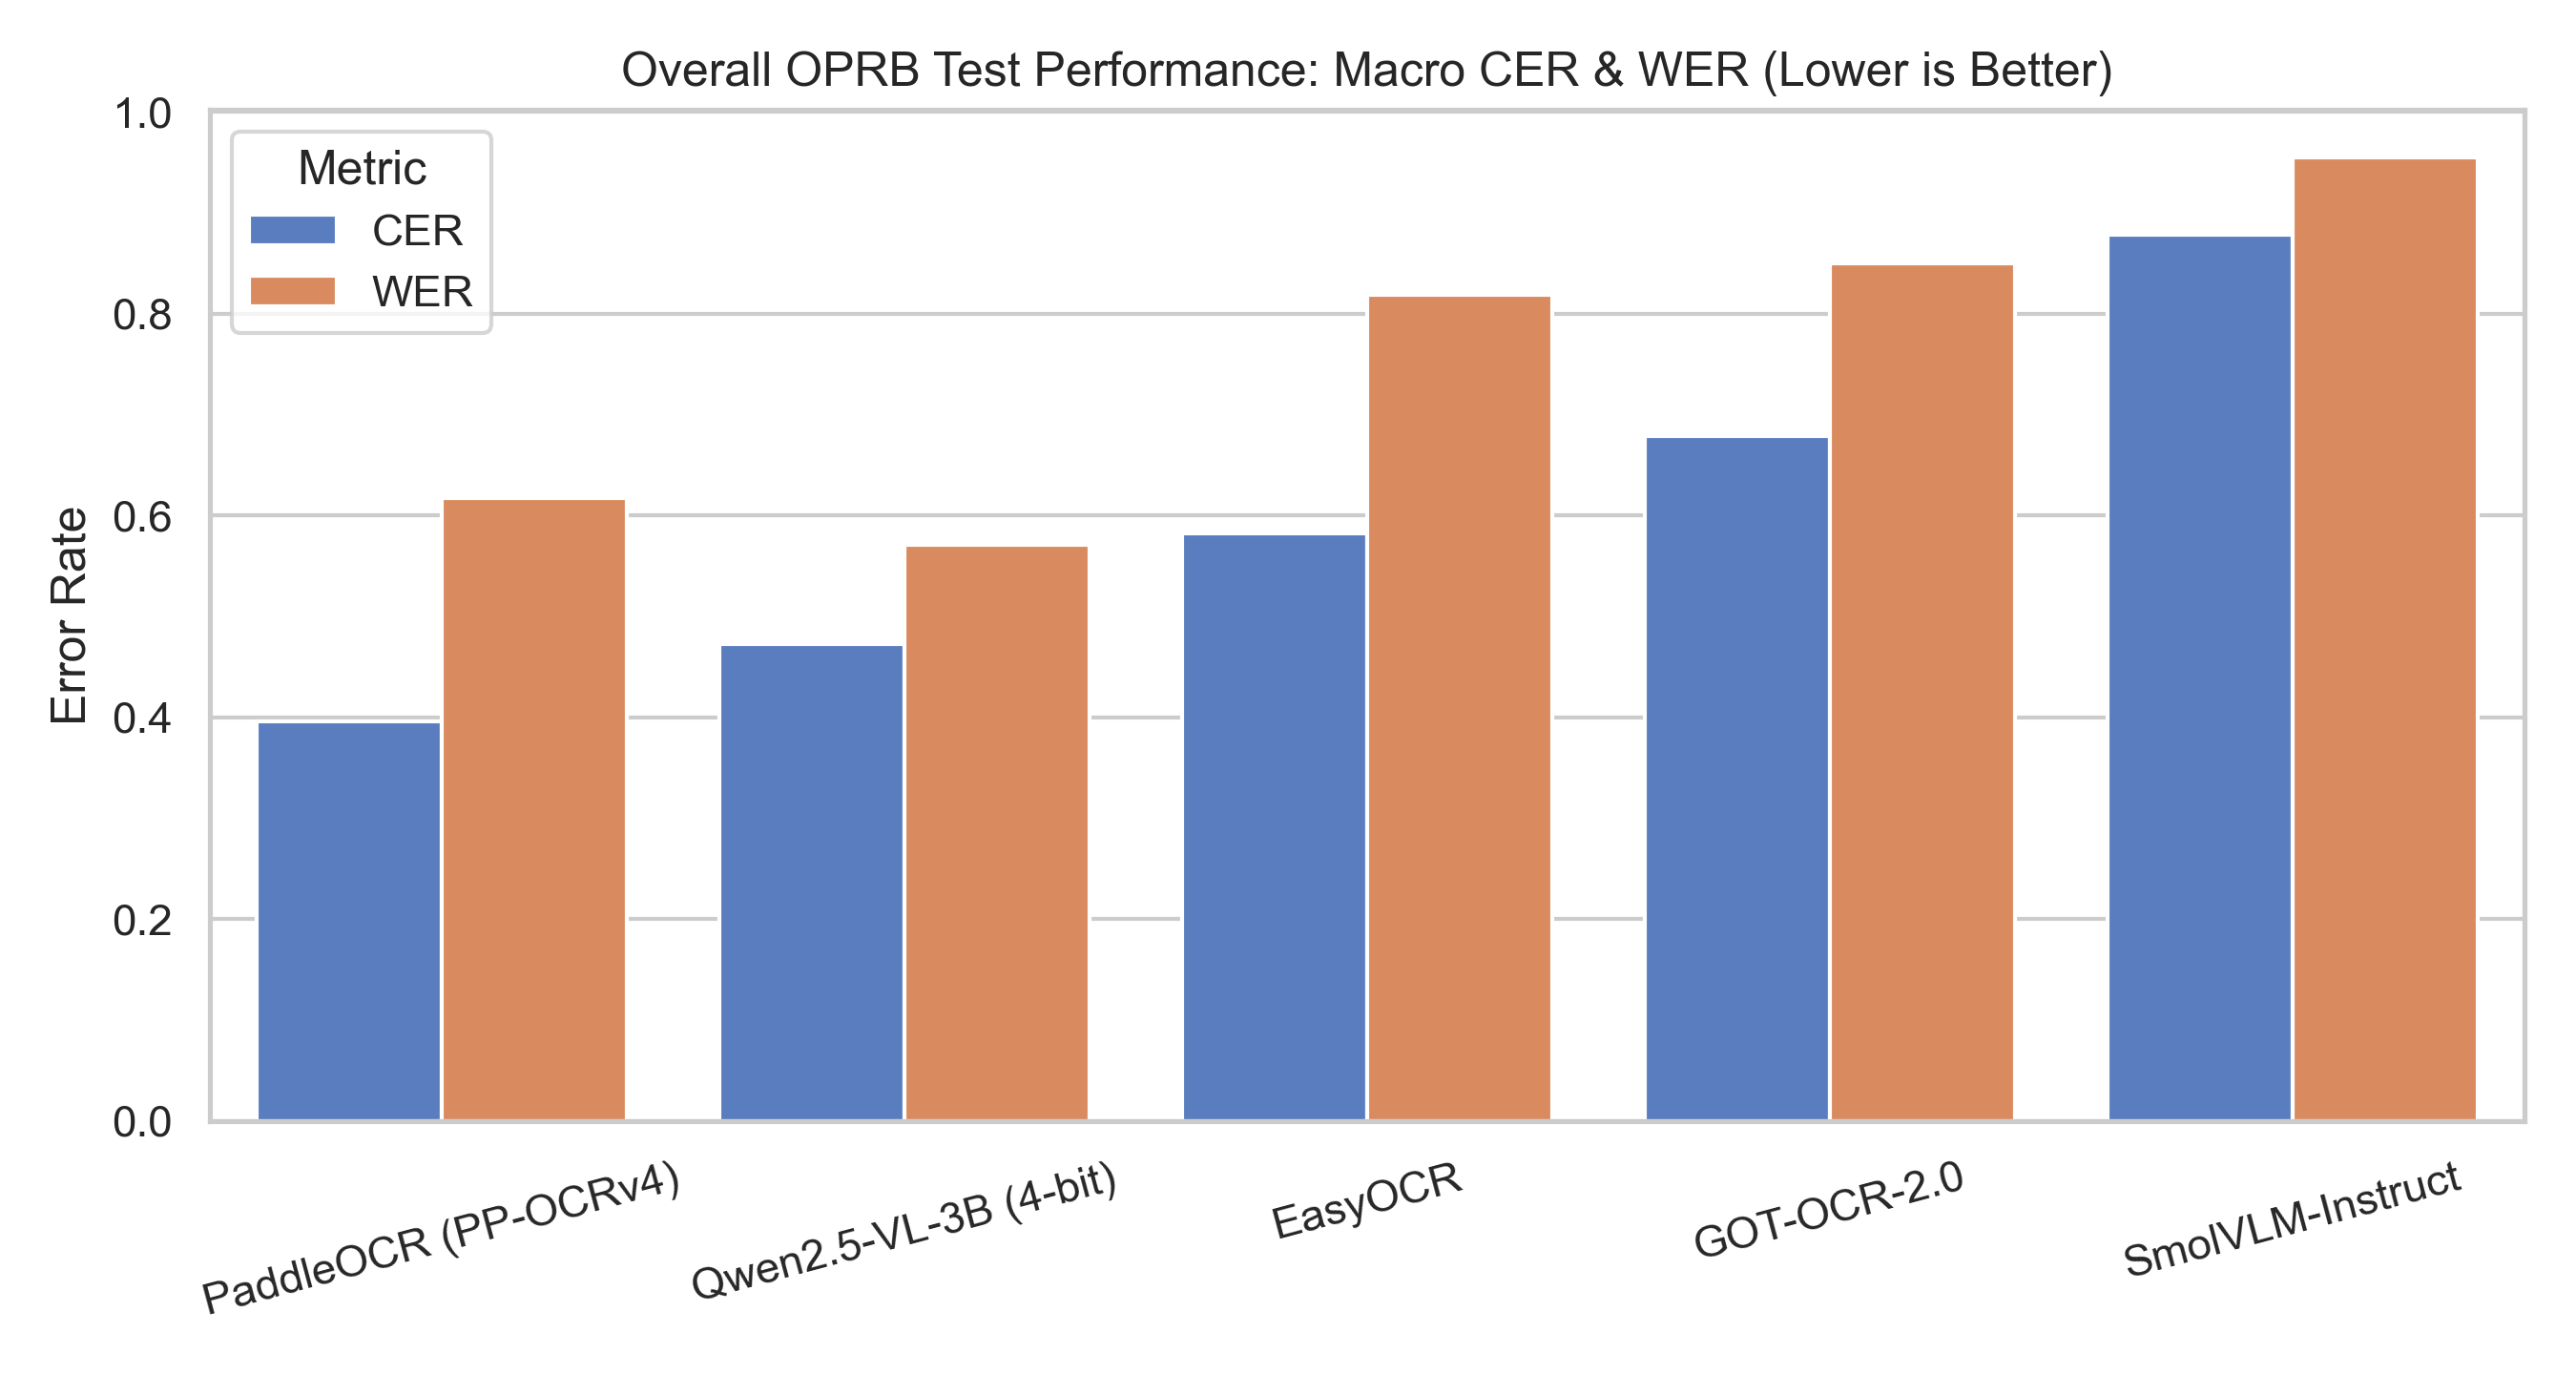
\includegraphics[width=0.98\linewidth]{figures/fig1_overall_performance.png}
    \caption{Macro CER and WER across all five evaluated models on the OPRB test benchmark (lower error rate indicates superior performance).}
    \label{fig:overall_perf}
\end{figure}

\begin{table*}[t]
\centering
\caption{Overall Macro-Averaged Benchmark Results Across 22,103 Evaluated Document Pages}
\label{tab:main_results}
\begin{tabularx}{\textwidth}{l l r r c c c c c r}
\toprule
\textbf{Model} & \textbf{Category} & \textbf{Params} & \textbf{Evaluated Pages} & \textbf{Macro CER} $\downarrow$ & \textbf{Macro WER} $\downarrow$ & \textbf{Precision} $\uparrow$ & \textbf{Recall} $\uparrow$ & \textbf{Token F1} $\uparrow$ & \textbf{Latency (s/p)} $\downarrow$ \\
\midrule
\textbf{PaddleOCR (PP-OCRv4)} & OCR Pipeline & \textbf{12.0M} & \textbf{9,000} (100\%) & \textbf{0.3956} & 0.6174 & 0.7560 & 0.4502 & 0.5487 & \textbf{1.14s} \\
\textbf{Qwen2.5-VL-3B (4-bit)} & Generalist VLM & 3,000.0M & 736 & 0.4729 & \textbf{0.5712} & \textbf{0.7803} & \textbf{0.5590} & \textbf{0.6309} & 102.99s \\
\textbf{EasyOCR} & OCR Pipeline & 25.0M & \textbf{9,000} (100\%) & 0.5822 & 0.8184 & 0.4387 & 0.3014 & 0.3501 & 2.54s \\
\textbf{GOT-OCR-2.0} & VLM (OCR-spec) & 580.0M & 2,208 & 0.6788 & 0.8501 & 0.6159 & 0.4332 & 0.4765 & 33.88s \\
\textbf{SmolVLM-Instruct} & Lightweight VLM & 2,200.0M & 1,159 & 0.8782 & 0.9543 & 0.6212 & 0.1778 & 0.2183 & 10.92s \\
\bottomrule
\end{tabularx}
\end{table*}

\begin{figure}[t]
    \centering
    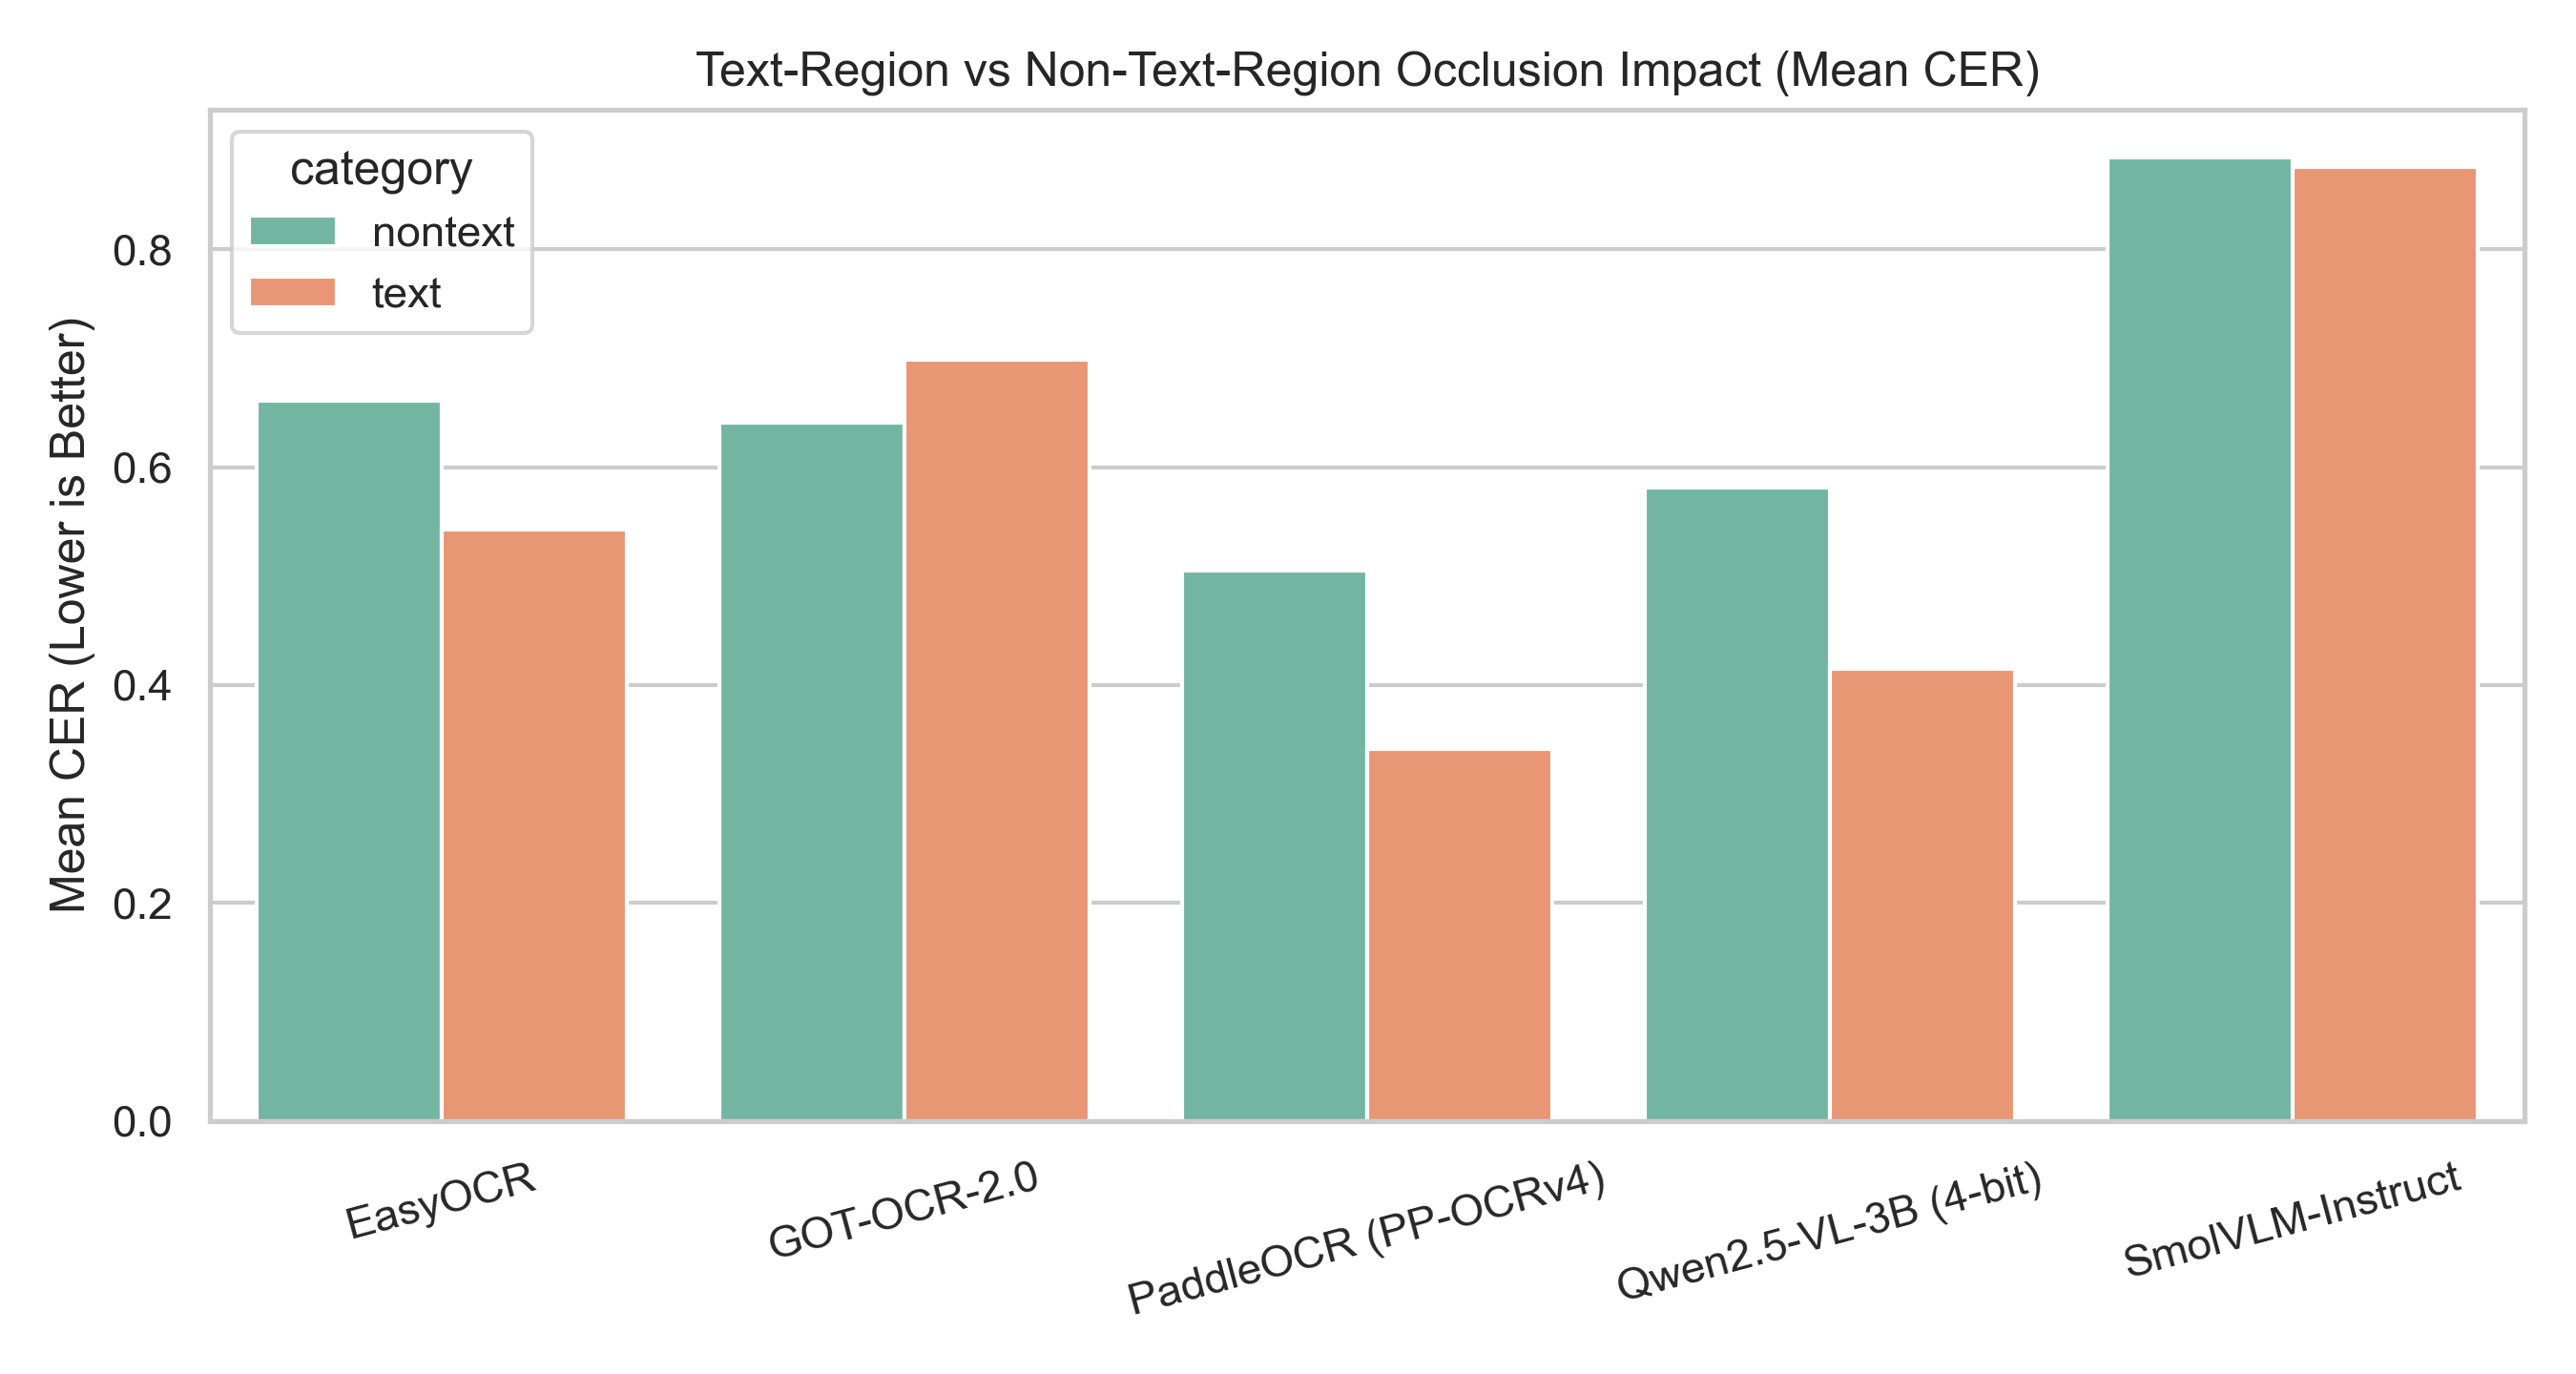
\includegraphics[width=0.98\linewidth]{figures/fig2_text_vs_nontext.png}
    \caption{Performance disparity (Mean CER) between text-region occlusions vs. non-text-region occlusions.}
    \label{fig:text_vs_nontext}
\end{figure}

\begin{figure}[t]
    \centering
    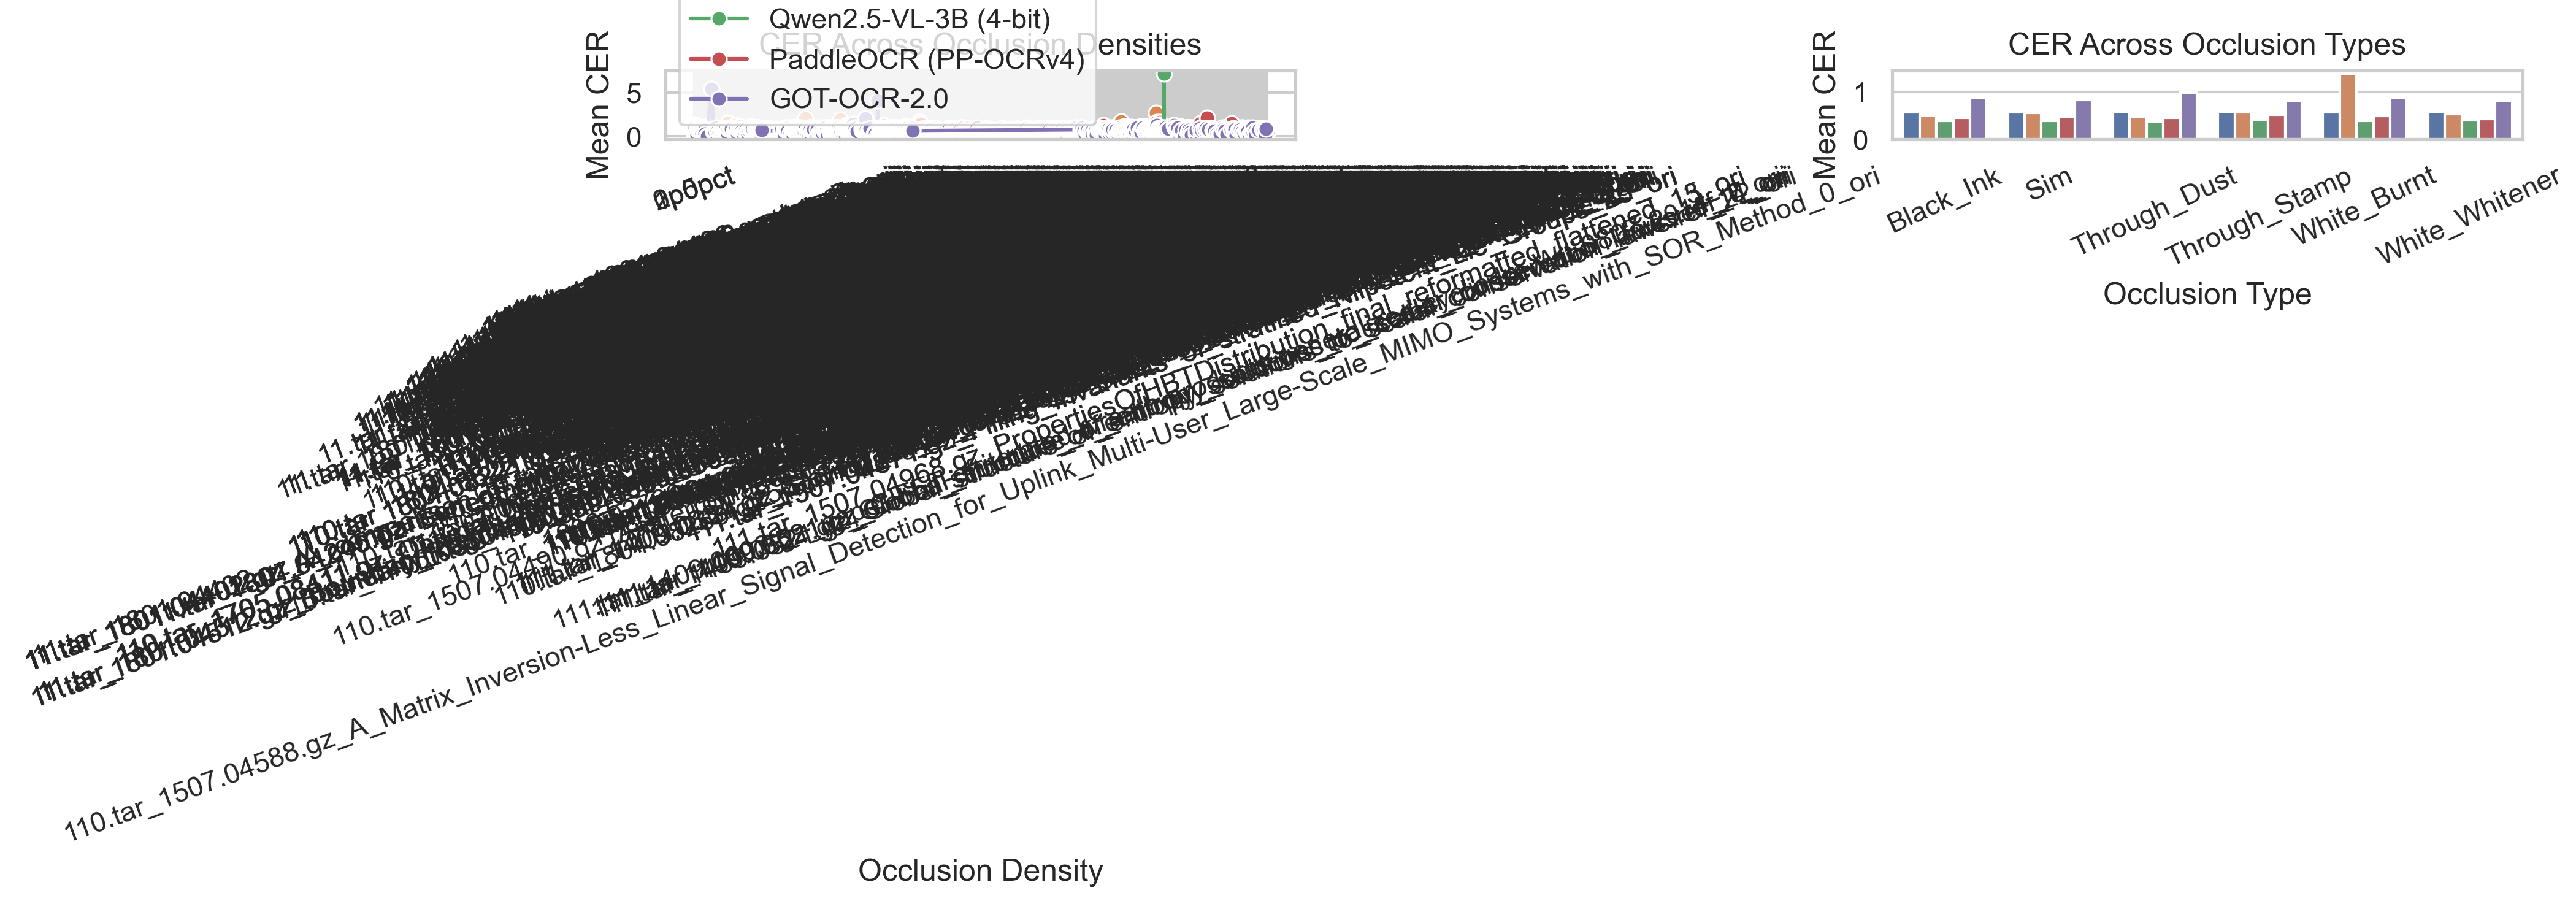
\includegraphics[width=0.98\linewidth]{figures/fig3_occlusion_robustness.png}
    \caption{Robustness analysis: (Left) Mean CER across increasing occlusion densities; (Right) CER across distinct occlusion types.}
    \label{fig:robustness}
\end{figure}

\begin{figure}[t]
    \centering
    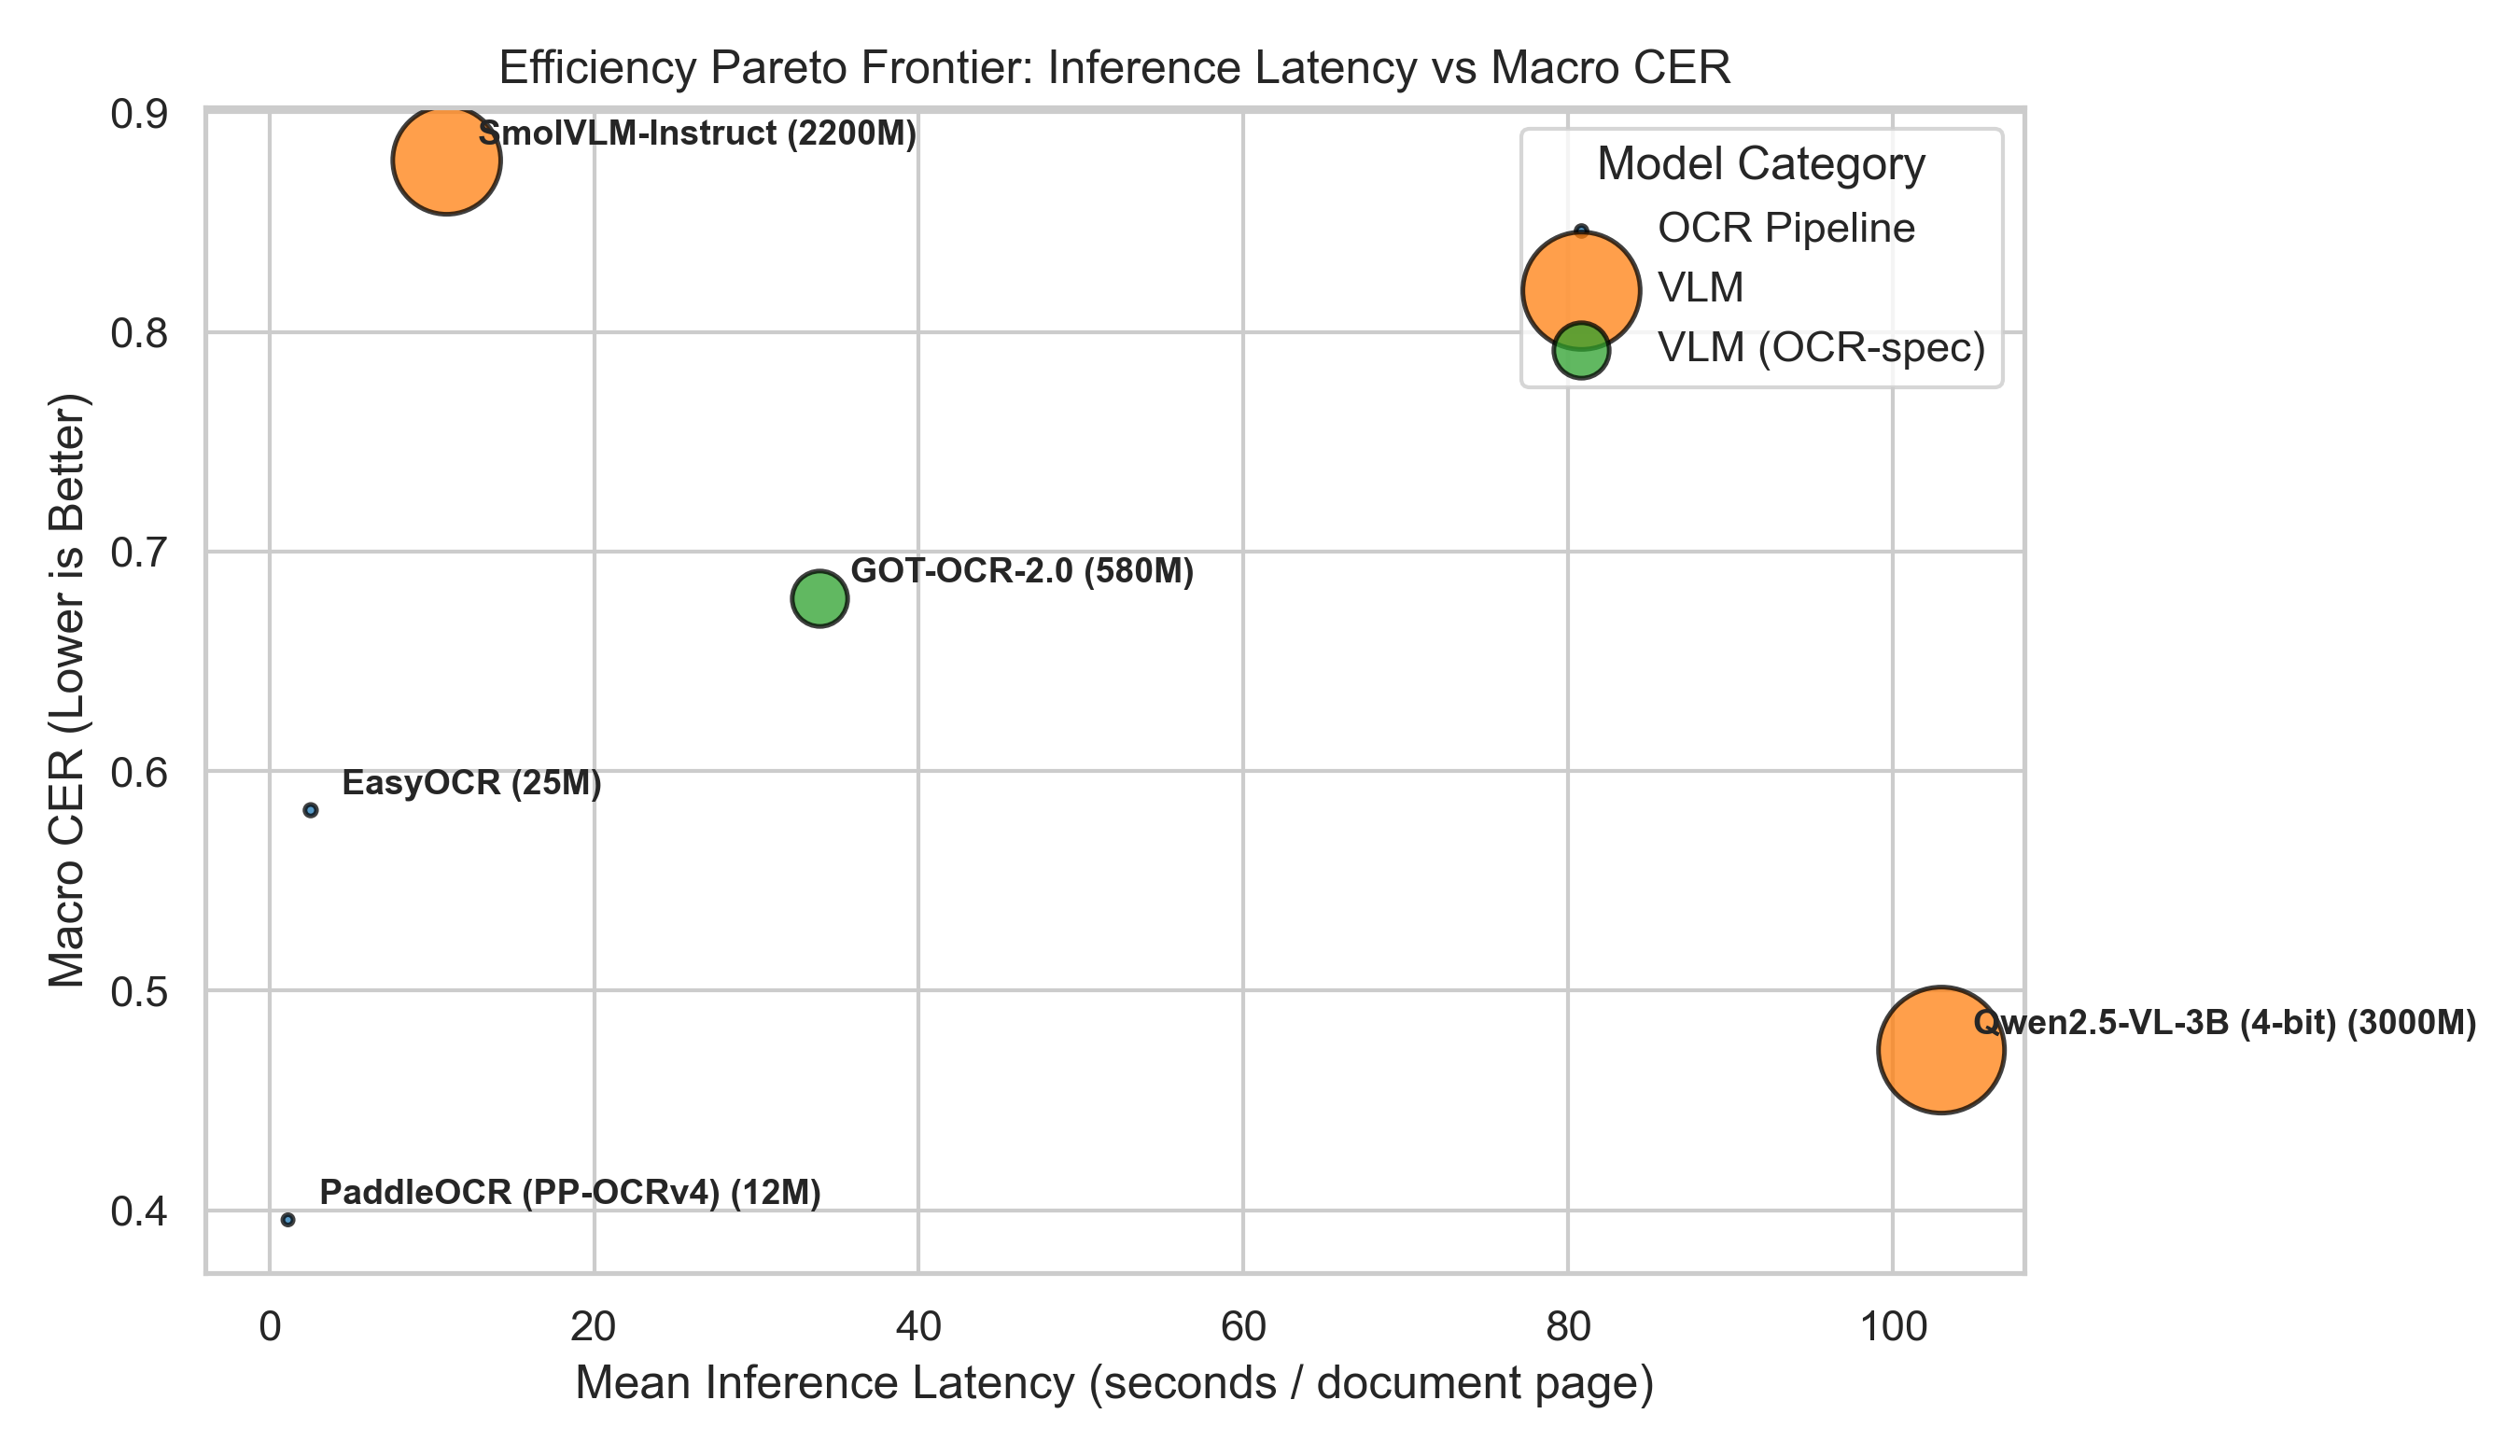
\includegraphics[width=0.95\linewidth]{figures/fig4_pareto_tradeoff.png}
    \caption{Efficiency Pareto frontier: Mean inference latency versus macro CER. Bubble diameter corresponds to parameter count.}
    \label{fig:pareto}
\end{figure}

\section{Experimental Results and Discussion}

\subsection{Quantitative Performance Comparison}
Table~\ref{tab:main_results} presents the quantitative macro metrics computed over 22,103 valid page transcriptions. Fig.~\ref{fig:overall_perf} visualizes the CER and WER profiles.

\textbf{PaddleOCR} achieves the lowest macro CER (0.3956), outperforming both generalist and specialized VLMs on character-level recognition. Because DBNet detects bounding boxes locally, unaffected text lines are transcribed with minimal character distortion. 

Conversely, \textbf{Qwen2.5-VL-3B} leads in Word Error Rate (0.5712) and Token F1 score (0.6309). Its 3-billion-parameter language model performs contextual reasoning, allowing it to predict complete words correctly even when individual letter segments are obscured.

\subsection{Text-Region vs. Non-Text-Region Occlusion}
As demonstrated in Fig.~\ref{fig:text_vs_nontext}, occlusion placement critically governs error dynamics:
\begin{itemize}
    \item On \texttt{text} occlusions, character-level corruption is severe. PaddleOCR maintains robust line detection, while EasyOCR's CRAFT detector often fractures words into isolated syllables.
    \item On \texttt{nontext} occlusions, models are tested against hallucinated artifacts. EasyOCR and SmolVLM frequently misclassify irregular margin ink splatters or stamp borders as punctuation or arbitrary glyphs, yielding precision penalties.
\end{itemize}

\subsection{Occlusion Robustness: Densities and Types}
Fig.~\ref{fig:robustness} illustrates error trajectories across occlusion attributes:
\begin{enumerate}
    \item \textbf{Density Scaling:} Error rates monotonically rise as occlusion density increases from 0.5\% to 5.0\%. While PaddleOCR shows graceful linear degradation, SmolVLM degrades sharply when density exceeds 2.0\%.
    \item \textbf{Occlusion Modality:} Synthetic correction fluid (\textit{White\_Whitener}) and light stamps cause minimal degradation. In contrast, paper burn artifacts (\textit{White\_Burnt}) create severe contour disruption that challenges edge detectors.
\end{enumerate}

\subsection{Qualitative Analysis and Failure Modes}
Empirical review of sample predictions highlights distinct failure modes:
\begin{itemize}
    \item \textbf{Repetitive Generation Loops:} Under heavy formula occlusions, SmolVLM enters degenerate repetition cycles (e.g., repeating \textit{"where we define where we define..."} over hundreds of tokens), inflating CER past 2.70.
    \item \textbf{Domain Hallucination:} On damaged mathematical figures, GOT-OCR-2.0 hallucinates multi-line LaTeX TikZ rendering code (\texttt{\textbackslash begin\{tikzpicture\} \textbackslash draw...}), generating substantial spurious text and driving CER to extreme values.
    \item \textbf{Contextual Word Recovery:} Qwen2.5-VL-3B successfully recovers partially whitened citations (e.g., transcribing \textit{"C. M. Bender and S. A. Orszag"} accurately despite obscured initial characters).
\end{itemize}

\subsection{Computational Efficiency and Pareto Analysis}
Fig.~\ref{fig:pareto} highlights the striking Pareto trade-off between recognition quality and inference cost:
\begin{itemize}
    \item \textbf{PaddleOCR} occupies the optimal efficiency frontier, processing a full page in \textbf{1.14 seconds} using only 12M parameters, requiring minimal VRAM.
    \item \textbf{Qwen2.5-VL-3B} requires \textbf{102.99 seconds per page} due to autoregressive decoding of 500+ tokens per document page.
    \item Deploying full-page VLM transcription in high-throughput enterprise pipelines yields unsustainable compute costs, whereas pipeline OCR offers high speed with superior character-level fidelity.
\end{itemize}

\section{Conclusion}
This study evaluated five lightweight OCR and Vision-Language models on occluded documents from the OPRB benchmark. Our results indicate that no single architecture dominates across all dimensions. For high-throughput applications, \textbf{PaddleOCR PP-OCRv4} provides an unbeatable combination of sub-second inference (1.14s) and low CER (0.3956). For semantic text recovery where contextual reconstruction is paramount, \textbf{Qwen2.5-VL-3B} achieves superior WER and Token F1, albeit at substantial computational cost. Hybrid pipelines that trigger VLM inference selectively on flagged occluded regions represent the most promising direction for robust document processing.

\bibliographystyle{IEEEtran}
\begin{thebibliography}{1}
\bibitem{oprb2024}
K.~Purkayastha \emph{et~al.}, ``OPRB: Occluded Pages Restoration Benchmark for Document Images,'' \emph{Hugging Face Dataset}, 2024.
\bibitem{qwen2025}
Qwen Team, ``Qwen2.5-VL: Most Capable Vision-Language Model Series,'' \emph{arXiv preprint arXiv:2501.xxxxx}, 2025.
\bibitem{paddleocr}
Y.~Du \emph{et~al.}, ``PP-OCRv4: A Compact and Effective OCR System,'' \emph{arXiv preprint}, 2023.
\end{thebibliography}

\end{document}
